\section{Auswahl der Skriptsprachen}
\setauthor{Robert Freiseisen}

Die Wahl der Scriptsprachen wurde auf Grund einer intensiven Internet-Recherchen 
und Fachgesprächen mit Mitschüler*innen und Professor*innen gefällt.\\
Folgende Scriptsprachen wurden gewählt:

\begin{itemize}
    \item Lua
    \begin{itemize}
        \item Lua wird oft als Modifikation für Videospiele, wie "Roblox" oder "World of Warcraft" eingesetzt.
        Zudem ist die Scriptsprache sehr einfach gehalten und daher schnell zu erlernen. 
        Ein gut dokumentiertes "Nuget-Paket" (Nlua), war das entscheinde Argument.
    \end{itemize}
    \item Python (IronPython)
    \begin{itemize}
        \item Nach Javascript ist Python, die meist genutzte Programmiersprache. Des wegen wurde sich für Python entschieden.
        Das Nuget-Paket "IronPython" wurde gewählt, da dieses Paket alle relevanten Funktionen von Python unterstützt.
        Außerdem ist "IronPython", das einzige Nuget-Paket, das die aktuellen .NET-Versionen unterstützt.
    \end{itemize}
    \item Csharpscript
    \begin{itemize}
        \item Csharp ist die populärste Programmiersprache im .NET-Bereich. Csharpscript unterstützt sowohl gehostete als auch eigenständige Ausführungsmodelle.
        Da Csharpscript ein eigen-entwickeltes "Nuget-Paket" zur Verfügung stellt, wurde auch dieses für die Arbeit genutzt.
    \end{itemize}
    \item Javascript
    \begin{itemize}
        \item Javascript ist eine weit verbreitete Programmiersprache. Also für jedes Projekt, dass Anpassungen anbieten möchte relevant.
        Zudem wurde Javascript im Unterrich erlernt.\\
        Die Wahl für das "Nuget-Packet" fiel auf "JavaScriptEngineSwitcher". \\ 
        Da es die meisten "Engines" für Javascript unterstützt.
    \end{itemize}
\end{itemize}

\section{Kriterienkatalog}
\setauthor{Robert Freiseisen}
Alle Daten wurden auf zwei unterschiedlichen Geräten gemessen. \\
Die Daten für IronPython und Lua wurden auf \\
PC A unter folgenden Voraussetzungen  gemessen:
\begin{itemize}
    \item Gerätspezifikationen:
    \begin{table}[H]
        \center
        \begin{tabular}{|p{3cm}|p{3cm}|}
            \hline
            Hersteller & HP \\ \hline
            Gerätname & LAPTOP-5U1879KR \\ \hline
            Prozessor & Intel(R) Core(TM) i5-8265U CPU @ 1.60GHz   1.80 GHz \\ \hline
            Installierter RAM & 8.00 GB (7.89 GB verwendbar) \\ \hline
            Produkt-ID & 00325-81357-65742-AAOEM \\ \hline
            Systemtyp & 64-Bit-Betriebssystem, x64-basierter Prozessor \\ \hline
        \end{tabular}
    \end{table}
    \item Betriebssystem:
    \begin{table}[H]
        \center
        \begin{tabular}{|p{4cm}|p{4cm}|}
            \hline
            Edition & Windows 11 Home \\ \hline
            Version & 21H2 \\ \hline
            Installiert am & 24.11.2021 \\ \hline
            Betriebssystembuild & 220.001.098 \\ \hline
            Leistung & Windows Feature Experience Pack 1000.22000.1098.0 \\ \hline
        \end{tabular}        
    \end{table}
\end{itemize}

\newpage
Die Daten für Csharpscript und Javascript wurden auf \\
PC B unter folgenden Voraussetzungen  gemessen:
\begin{itemize}
    \item Gerätspezifikationen:
    \begin{table}[H]
        \center
        \begin{tabular}{|p{3cm}|p{3cm}|}
            \hline
            Hersteller & Acer \\ \hline
            Gerätname & Beptop \\ \hline
            Prozessor & Intel(R) Core(TM) i5-8265U CPU @ 1.60GHz \\ \hline
            Installierter RAM & 16.00 GB (15.9 GB verwendbar) \\ \hline
            Produkt-ID & C125C288-8DFB-4042-A3BA-EE3236D35AB7 \\ \hline
            Systemtyp & 64-Bit-Betriebssystem, x64-basierter Prozessor \\ \hline
        \end{tabular}
    \end{table}
    \item Betriebssystem:
    \begin{table}[H]
        \center
        \begin{tabular}{|p{4cm}|p{4cm}|}
            \hline
            Edition & Windows 11 Home \\ \hline
            Version & 21H2 \\ \hline
            Installiert am & 06.10.2021 \\ \hline
            Betriebssystembuild & 220.001.098 \\ \hline
            Leistung & Windows Feature Experience Pack 1000.22000.1098.0 \\ \hline
        \end{tabular}        
    \end{table}
\end{itemize}


\newpage
\subsection{Aktivität der Entwicklung}

In der nachfolgenden Tabelle wird dargestellt, wie intensiv die Entwicklerteams an den unterschiedlichen Scriptsprachen arbeiten und ob diese auch die Nuget-Pakete entwickeln.
\begin{table}[H]
    \begin{tabular}{|p{3cm}|p{3cm}|p{3cm}|p{3cm}|p{3cm}|}
        \hline
        Aktivität & IronPython & Lua & CsharpScripting & Javascript\\ \hline
        Commits in den letzten 10 Monaten & 179 & 27 & 702 & 1153 \\ \hline
        Nuget-Packages vom Sprach-entwicklerteam selber &Nein &Nein &Ja & Nein\\ \hline
        Releases in den letzten 10 Monaten & 2 (2.7.1 und 3.4.0-beta1) & 1 (v5.4.4) & v4.0.0 und höher & v4.6.2 (und höher)\\ \hline
        Unterstützt aktuelle major Versionen von Scriptsprache & Ja & Ja & Ja & Ja\\ \hline
        Unterstützt aktuelle Versionen von .NET & Ja & Ja & Ja & Ja \\ \hline
    \end{tabular}
\end{table}
\newpage
\subsection{Einsetzbarkeit}
Die folgende Tabelle stellt dar, auf welchen Betriebssystemen die veschiedenen Scriptsprachen mit .NET lauffähig sind.

\begin{table}[H]
    \center
    \begin{tabular}{|p{3cm}|p{3cm}|p{3cm}|p{3cm}|p{3cm}|}
        \hline
        Einsetzbarkeit & IronPython & Lua & CsharpScripting & Javascript\\ \hline
        Auf Windows lauffähig & Ja & Ja & Ja & Ja \\ \hline
        Auf MAC lauffähig & Ja & Ja & Ja & Ja \\ \hline
        Auf Linux lauffähig & Ja & Ja & Ja & Ja \\ \hline
 
    \end{tabular}
\end{table}
\newpage
\subsection{Performance}
Der Speicherplatzt wurde aus dem Windows-File-Explorer entnommen. 
Die Geschwindigkeitsmessungen erfolgten mit Dotnet-Benchmark.

Dotnet-Benchmark ist ein Framework dass ein Codeabschnitt mehrfach hintereinander ausführt 
und somit eine Statistik über Diesen erstellt. Diese Statistik kann man auf verschiedene Arten exportieren, wie zum Beispiel als CSV-Datei oder als Textdatei.

Als eine einfache Anwendung wird ein Programm genommen, dass eine Funktion aufruft, welche 42 zurück gibt 
und dies anschließen auf die Konsole ausgibt.
\begin{table}[H]
    \begin{tabular}{|p{3cm}|p{3cm}|p{3cm}|p{3cm}|p{3cm}|}
        \hline
        Performance & IronPython & Lua & CsharpScripting & Javascript\\ \hline
        Speicher einer einfachen Anwendung & 13 MB & 7.3 MB & 168 KB & 416 KB  \\ \hline
        Durchnittliche Laufzeit einer einfachen Anwendung & 137.118 $\mu$s & 8.088 $\mu$s & 90.24 $\mu$s & 31.65 $\mu$s \\ \hline
        Durchnittliche Laufzeit einer Additionsfunktion & 2340.688 $\mu$s & 10.053 $\mu$s & 83.82 $\mu$s & 16.03 $\mu$s \\ \hline
        Durchnittliche Laufzeit von Übergabe eines .NET-Objekts & 9054.007 $\mu$s & 7548.497 $\mu$s &  & \\ \hline
    \end{tabular}
\end{table}

\newpage
Es folgen nun die Resultate von Dotnet-Benchmark:
\linebreak
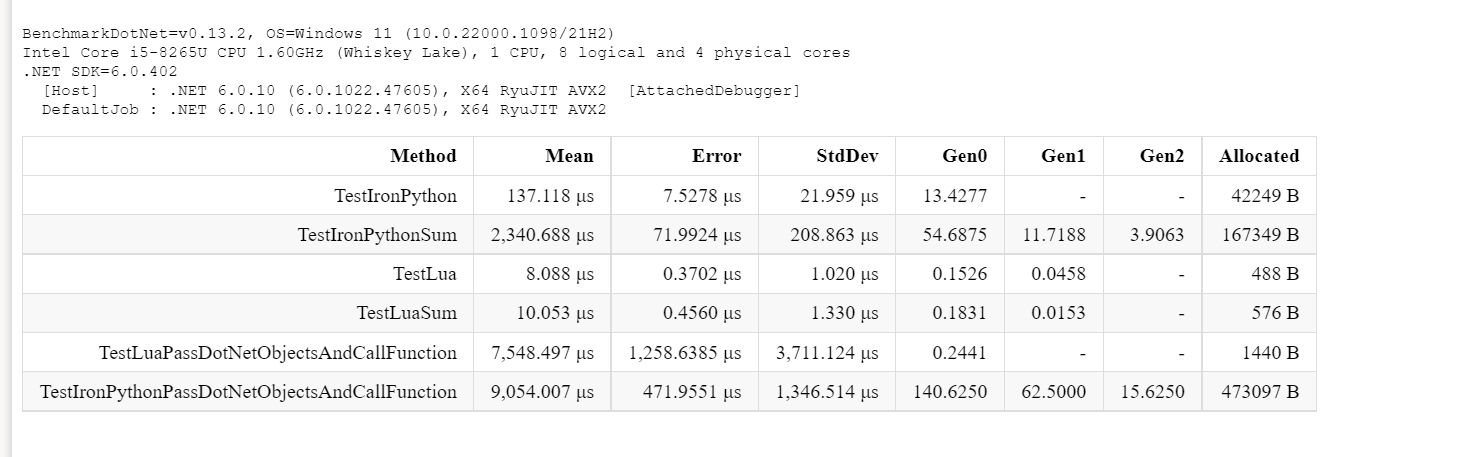
\includegraphics[scale=0.5]{pics/benchmark_results_NluaVsIronPython.png}
\linebreak
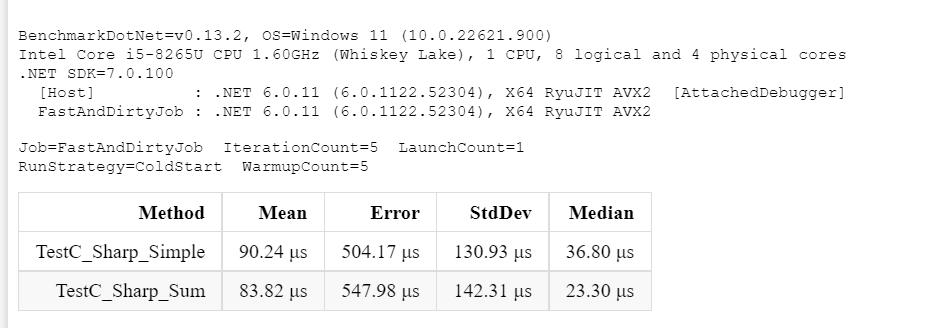
\includegraphics[scale=0.5]{pics/benchmark_results_csharpScript.png}
\linebreak
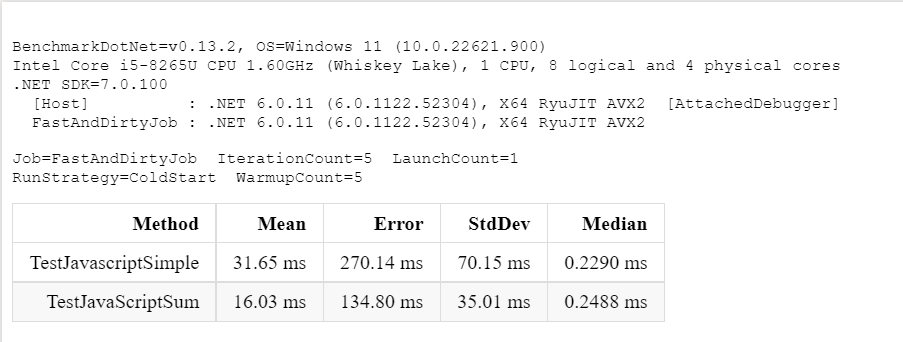
\includegraphics[scale=0.5]{pics/benchmark_results_javascript.png}
\newpage
\subsection{Funktionalität}
In der nachfolgenden Tabelle sind die Recherche-Ergebnisse hinsichtlich der Funktionalität der Scriptsprachen in .NET dargestellt.
Die Informationen wurden aus den offizellen Webseiten der Nuget-Pakete entnommen.

\begin{table}[H]
    \begin{tabular}{|p{3cm}|p{3cm}|p{3cm}|p{3cm}|p{3cm}|}
        \hline
        Funktion & IronPython & Lua & CsharpScripting & Javascript\\ \hline
        Kann auf .NET Variablen zugreifen & Ja & Ja & Ja & Ja \\ \hline
        Kann globale Variablen & Ja & Ja & Ja & Ja \\ \hline
        Unterstützt Erweiterungspakete der Scriptsprache & Ja (nicht numpy und pandas!) & Ja & Ja & Ja \\ \hline 
    \end{tabular} 
\end{table}
\newpage
\subsection{Debugging}
In der nachfolgenden Tabelle ist dargestellt, welche Art des Debugging bei welcher Scriptsprache möglich ist.

\begin{table}[H]
    \begin{tabular}{|p{2.5cm}|p{2.5cm}|p{2.5cm}|p{2.5cm}|p{2.5cm}|}
        \hline
        Debugging & IronPython & Lua & CsharpScripting & Javascript\\ \hline
        Debugging durch Ausgabe auf der Konsole & Ja & Ja & Ja & Ja \\ \hline
        Debugging mit Break Points in Visual Studio & Ja & Nein & Nein & Nein\\ \hline
        Debugging mit Break Points in Visual Studio Code & Ja & Nein & Nein & Nein \\ \hline
    \end{tabular}
\end{table}